\documentclass[crop,tikz]{standalone}
\usepackage{tikz}
\usetikzlibrary{shapes, snakes}
\begin{document}

\def\p{0.1}

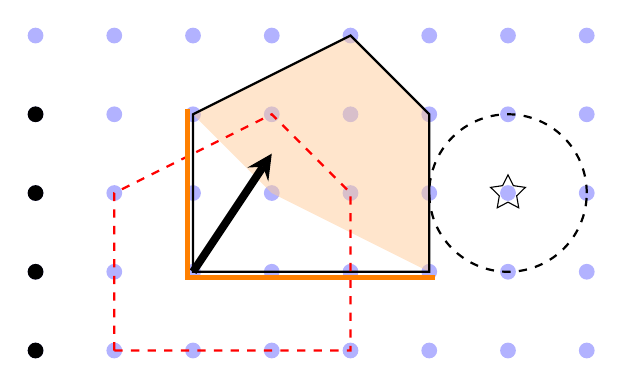
\begin{tikzpicture}[
    point/.style={draw=none, circle, fill=blue!30, minimum width=0.2cm, inner sep=0, outer sep=0}
]
    \foreach \x in {0,...,7}
        \foreach \y in {0,...,4} 
            \node [point] (\x\y) at (\x, \y) {};
            
    \foreach \point [count=\i] in {(0, 0), (0, 1), (0, 2), (0, 3)} {
        \node [point, fill=black] () at \point {};
    }
    
    \filldraw[draw=none, thick, rounded corners=0mm, opacity=0.5, inner sep=10mm, color=black, fill=orange!40] (3, 2) -- (2,3) -- (4,4) -- (5,3) -- (5,1) -- cycle;
    
    \draw[thick, rounded corners=0mm, inner sep=10mm] (2, 1) -- (2,3) -- (4,4) -- (5,3) -- (5,1) -- cycle;
    
    \draw[thick, rounded corners=0mm, dashed, inner sep=10mm, color=red] (1, 0) -- (1,2) -- (3,3) -- (4,2) -- (4,0) -- cycle;
    
    \draw[-stealth, line width=1mm] (2, 1) -- (3,2.5);
    
    \node[circle, draw, thick, dashed, minimum width=2cm] () at (6,2){};
    \node[star, star points=5, draw, star point ratio=2, scale=0.7] () at (6,2){};
    
    \draw[orange, ultra thick] (23.north west) -- (21.south west) -- (51.south east);
\end{tikzpicture}
\end{document}